% =====================================================================
% Chapter 5 -- Method
%
% Outline: outlines/ch5_method.md (approved 2026-10-21).
% Facts: thesis_notes.md §2 "Method fact sheet" (from code/, run configs and logs),
% paper_notes/{voxtell,zscl,cpe_clip}.md. Notation: thesis_notes.md §5.
% Values of all parameters belong to Ch. 6; this chapter uses symbols.
% Every paragraph marked CLAUDE-DRAFT is to be rewritten by the author.
% =====================================================================

\chapter{Method}
\label{chap:method}

% CLAUDE-DRAFT
This chapter describes what we built to answer the research question and why.
\Cref{sec:method-setting} defines the continual-learning setting, \cref{sec:method-protocol} the protocol that measures adaptation and forgetting, \cref{sec:method-adaptation} how VoxTell is adapted to a single task, \cref{sec:method-strategies} the strategies built on this procedure, and \cref{sec:method-complexity} their computational cost.
The concepts are introduced in \cref{chap:background}; the values of all parameters and the experiments follow in \cref{chap:experiments}.

% ---------------------------------------------------------------------
\section{Continual-Learning Setting}
\label{sec:method-setting}

% CLAUDE-DRAFT
We consider a sequence of $T = 6$ tasks built from SKM-TEA.
Each task $t \in \{1, \dots, T\}$ is defined by one knee structure, its text prompt $p_t$ and the binary masks of that structure (\cref{tab:ch4_structures}).
We write $\mathcal{D}_t^{\mathrm{tr}}$, $\mathcal{D}_t^{\mathrm{val}}$ and $\mathcal{D}_t^{\mathrm{te}}$ for the training, validation and test sets of task~$t$, each consisting of the volumes of the corresponding split (\cref{sec:data-splits}) paired with the masks of structure~$t$.
The model is trained on task~1, then on task~2, and so on, and after training on task~$t$ it should still segment the structures of tasks $1, \dots, t-1$ when given their text prompts.
Because all six tasks share the same volumes, the images do not change from one task to the next.
What changes is the target: every task introduces a new structure, with its own masks and its own text prompt.
Catastrophic forgetting therefore shows up here as a loss of segmentation performance on earlier structures in the same images.

% CLAUDE-DRAFT
In every strategy, the text prompt names the target structure during training and at inference.
Only task-specific LoRA (\cref{subsec:method-lora}) additionally receives the task identity~$t$ at inference and uses it to select parameters trained for that task (task-aware inference, \cref{sec:bg-cl}); all other strategies use one parameter set for all tasks.

% CLAUDE-DRAFT
The protocol has two variables that are set per run.
The first is the task order: a run trains all tasks in one fixed order, and comparing runs that differ only in the task order shows whether the results depend on the order in which the structures are learned.

% CLAUDE-DRAFT
The second variable is the amount of labelled data.
In a few-shot setting, every task is trained on the first $k$ volumes of its training split (\cref{sec:data-splits}) instead of on the full split, and we refer to $k$ as the number of shots, that is, the number of labelled training volumes per task.
Within a run, $k$ is the same for all tasks, and the validation and test sets do not depend on~$k$.
The task orders and values of $k$ that we used, and the reasons for them, are given with the experiments in \cref{subsec:exp-data}.

% CLAUDE-DRAFT
In addition to the six tasks, we evaluate a control task that is not part of the task sequence and is never trained on: segmentation of the lung in the AeroPath test volumes $\mathcal{D}_c^{\mathrm{te}}$ with the text prompt $p_c = $ ``lung''.
It measures how much of VoxTell's pretrained ability on structures outside the task sequence is lost during adaptation, following the control set of SPU~\cite{Zhang_2024_CVPR}.
We chose this task for two reasons.
Lung is a concept that VoxTell knows well from its training data, while AeroPath itself was not used for training (\cref{sec:data-aeropath}), and the pretrained model segments it with a mean \gls{dsc} of 0.979 on our four test volumes (\cref{fig:ch6_control_task_main}), so a loss of ability is clearly visible.
In addition, AeroPath is publicly available.

% ---------------------------------------------------------------------
\section{Evaluation Protocol}
\label{sec:method-protocol}

% CLAUDE-DRAFT
The protocol trains a strategy on the $T$ tasks in sequence and evaluates the model after every training stage on every task and on the control task (\cref{alg:protocol}).
Stage $j = 0$ is the pretrained model with parameters $\theta_0$, and stage $j = t$ is the model after training on task~$t$.
After each stage~$j$, we record the mean \gls{dsc} $a_{i,j}$ on the test set $\mathcal{D}_i^{\mathrm{te}}$ of every task $i \in \{1, \dots, T\}$ and the mean \gls{dsc} $c_j$ on the control task.
The values $a_{i,j}$ form the evaluation matrix with $T$ rows and $T+1$ columns (\cref{sec:bg-cl}), and the values $c_j$ form an additional control row.
We evaluate all tasks at every stage, including tasks that have not been trained yet ($i > j$), because these entries show how training on one structure affects the segmentation of structures that come later in the sequence.
All metrics of this thesis are computed from these two quantities; their definitions are given in \cref{sec:bg-metrics}, and \cref{subsec:exp-metrics} explains which of them we report and why.

% CLAUDE-DRAFT
Each entry is the mean over the volumes of one test set of the per-volume \gls{dsc} between the binary prediction and the label mask, with the prediction obtained by sliding-window inference (\cref{sec:method-adaptation}).
Every entry of every run uses the same test volumes: the 24 SKM-TEA test volumes for the tasks and the 4 AeroPath test volumes for the control task (\cref{sec:data-splits}).
Differences between entries, and between runs, therefore never come from different test data.
We also keep the per-volume values, from which \cref{subsec:exp-metrics} estimates the variability of the metrics over test volumes.

% CLAUDE-DRAFT
Which parameters are evaluated at stage~$j$ depends on the strategy.
All strategies except task-specific LoRA evaluate one parameter set, obtained after training on task~$j$, on every task and on the control task.
Task-specific LoRA holds one adapter per trained task and uses the task identity to choose among them (\cref{subsec:method-lora}): a task $i \le j$ is evaluated with the adapter trained on task~$i$, a task $i > j$ with the adapter of the current task~$j$, and the control task with the pretrained model without any adapter.
As a consequence, the entries of an earlier task do not change once its adapter is trained, and the control task always gives the pretrained result.
Low forgetting and the absence of a control-task drop are thus properties of this evaluation for task-specific LoRA, not measured effects.\todo{defense: task-specific LoRA's forgetting and control-task drop are zero by construction; state this wherever its results are compared}

% CLAUDE-DRAFT
As a reference, we apply the same metrics to the pretrained model itself, treating it as if it had been evaluated unchanged after every stage, that is, with $a_{i,j} = a_{i,0}$ and $c_j = c_0$ for all~$j$.
This pretrained-model reference shows whether a strategy moved away from the pretrained model at all and in which direction.
Because the order of the columns matters for some metrics, we compute it once for each task order.

% CLAUDE-DRAFT
As an upper reference, we train joint fine-tuning, which trains one model on the training sets of all six tasks at once, in a single stage.
Each training sample keeps the text prompt of its own structure, and all other settings are those of sequential fine-tuning (\cref{sec:method-adaptation}), so the joint model receives the same number of updates as sequential fine-tuning over the whole sequence.
It is evaluated on the test set of every task and on the control task after its single stage.
Without a task sequence, Adaptation, Final Forgetting and Transfer are not defined for it, so we compare it with the strategies on Final Performance, per structure and on the control-task drop.
We do not compute the intransigence measure of Chaudhry et al.~\cite{Chaudhry_2018}, because its reference for task~$k$ is a model trained jointly on tasks $1, \dots, k$, and our joint model, trained on all six tasks, provides this reference only for $k = T$.

\begin{algorithm}[tb]
\caption{Continual adaptation and evaluation protocol. \textsc{Adapt} adapts the model to one task (\cref{alg:adapt}); \textsc{Select} returns the parameters a strategy evaluates on a given task (the parameters of the stage for all strategies except task-specific LoRA, see text); \textsc{Evaluate} returns the mean \gls{dsc} over a test set.}
\label{alg:protocol}
\begin{algorithmic}[1]
\REQUIRE pretrained parameters $\theta_0$; strategy $\mathcal{S}$; tasks $t = 1, \dots, T$ in the chosen task order, each with text prompt $p_t$ and sets $\mathcal{D}_t^{\mathrm{tr}}, \mathcal{D}_t^{\mathrm{val}}, \mathcal{D}_t^{\mathrm{te}}$; control task with $p_c$ and $\mathcal{D}_c^{\mathrm{te}}$
\ENSURE evaluation matrix $(a_{i,j})$ with $i = 1, \dots, T$, $j = 0, \dots, T$; control row $(c_j)$
\STATE $\tilde{\theta}_0 \gets \theta_0$
\FOR{$j = 0$ \TO $T$}
  \IF{$j > 0$}
    \STATE $(\theta_j, \tilde{\theta}_j) \gets \textsc{Adapt}(\theta_{j-1}, j, \mathcal{S})$ \COMMENT{carried-forward and evaluated parameters}
  \ENDIF
  \FOR{$i = 1$ \TO $T$}
    \STATE $a_{i,j} \gets \textsc{Evaluate}(\textsc{Select}(\mathcal{S}, \tilde{\theta}_{0:j}, i), p_i, \mathcal{D}_i^{\mathrm{te}})$
  \ENDFOR
  \STATE $c_j \gets \textsc{Evaluate}(\textsc{Select}(\mathcal{S}, \tilde{\theta}_{0:j}, c), p_c, \mathcal{D}_c^{\mathrm{te}})$
\ENDFOR
\end{algorithmic}
\end{algorithm}

% CLAUDE-DRAFT
\Cref{alg:protocol} distinguishes the parameters $\theta_j$ that are carried forward to the next task from the parameters $\tilde{\theta}_j$ that are evaluated.
In the main evaluation, both are the parameters after the last epoch of task~$j$; the distinction matters for the two additional evaluations of \cref{sec:method-adaptation}, which evaluate the checkpoint with the lowest validation loss and, for the distillation-based strategy, the weight ensemble.

% CLAUDE-DRAFT
The cost of the protocol consists of $T$ calls of \textsc{Adapt}, whose cost is given in \cref{sec:method-adaptation}, and of the evaluations.
With $T+1$ stages, each evaluated on $T$ task test sets and the control test set, the protocol runs sliding-window inference on $(T+1)\,(T\,|\mathcal{D}^{\mathrm{te}}| + |\mathcal{D}_c^{\mathrm{te}}|)$ volumes, where $|\mathcal{D}^{\mathrm{te}}|$ is the size of a task test set; for our sets this is $7 \cdot (6 \cdot 24 + 4) = 1036$ volume inferences per run, and the same number again for each additional evaluation.
The evaluation time thus grows quadratically with the number of tasks, while the training time grows linearly.
Evaluation needs memory for one parameter set and the prediction of one volume at a time; the stored results are the $(T+1)^2$ means plus the per-volume values.
The measured evaluation time per volume and per run is reported in \cref{sec:exp-compute}.

% ---------------------------------------------------------------------
\section{Adapting VoxTell to One Task}
\label{sec:method-adaptation}

% CLAUDE-DRAFT
All strategies adapt VoxTell to a task with the same procedure, \textsc{Adapt} in \cref{alg:adapt}.
A strategy changes this procedure at three defined points, which we describe in \cref{sec:method-strategies}; this section describes the procedure itself.

% CLAUDE-DRAFT
We start every run from the released VoxTell checkpoint (version~1.1)~\cite{rokuss2025voxtellfreetextpromptableuniversal}, whose architecture is introduced in \cref{subsec:bg-voxtell}.
We use VoxTell because it accepts free-text prompts and reached the highest mean zero-shot \gls{dsc} in the comparison of its authors, ahead of SAT (\cref{sec:text-promptable-seg}).
\Cref{fig:ch5_voxtell} shows the model as it is used here, together with the parts that the strategies change.
Two properties of the implementation matter for what follows and differ from the description in the VoxTell paper.
First, the prompt decoder takes its keys and values from the output of encoder stage~4, which has $12^3$ voxels for a $192^3$ input patch, and not from the bottleneck.
Second, each of the $L_{\mathrm{dec}}$ prompt-decoder layers applies only a cross-attention block and a feed-forward block, each preceded by layer normalisation and followed by a residual connection.
Every layer also contains a self-attention module, but the configuration of the released model never executes it, so its parameters are never updated.
Before the first layer, the text embedding and the stage-4 features are projected to the model dimension~$d$ of the prompt decoder, and after the last layer one multilayer perceptron per decoder stage maps the output to the guidance~$\mat{E}_s$ of that stage, $s = 0, \dots, 4$.
At stages~4 to~1, the guidance is split into $G$ vectors whose dot products with the decoder features at every voxel are appended as $G$ new channels; at stage~0, the full resolution, a single dot product yields the output logits.
The text query $\vec{q}$ that enters the prompt decoder is the embedding of the text prompt computed by the text encoder Qwen3-Embedding-4B~\cite{zhang2025qwen3embedding}, which stays frozen in every strategy.

\begin{figure}[tb]
\centering
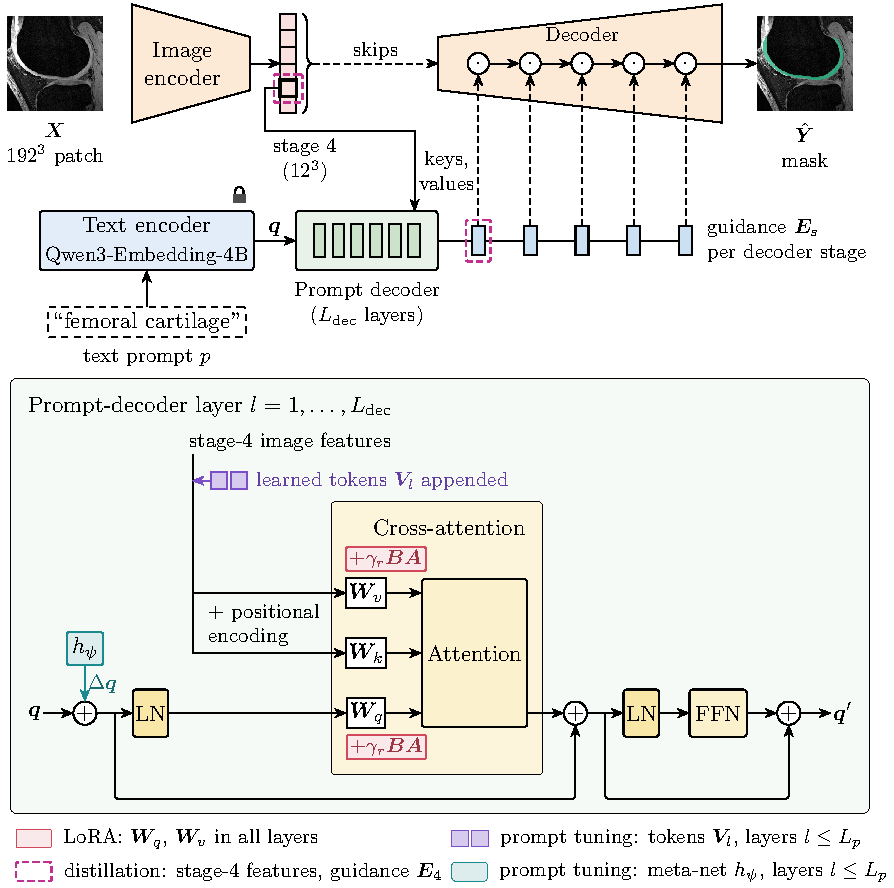
\includegraphics{figures/ch5_voxtell_strategies.pdf}
% CLAUDE-DRAFT
\caption[VoxTell as used in this thesis and the parts changed by the strategies]{VoxTell as used in this thesis and the parts that the continual-learning strategies change (layout adapted from~\cite[Fig.~2]{rokuss2025voxtellfreetextpromptableuniversal}).
Top: all encoder stages feed the decoder stage of the same resolution; the prompt decoder attends to the stage-4 features, and its output is mapped to the guidance~$\mat{E}_s$ of the five fusion points. The lock marks the frozen text encoder; the output panel shows the reference mask of femoral cartilage (test volume MTR\_005) for illustration.
Bottom: one prompt-decoder layer as executed; the attention block includes the output projection.
The coloured marks are explained in \cref{sec:method-strategies}. Sequential fine-tuning and the distillation-based strategy update all parameters except the text encoder; replay changes only the training data.}
\label{fig:ch5_voxtell}
\end{figure}

% CLAUDE-DRAFT
Training uses patches of $192^3$ voxels, the patch size of VoxTell.
In every epoch, each training volume contributes one patch: with probability $\pi_{\mathrm{fg}}$ the patch is centred on a voxel drawn at random from the target structure, otherwise it is placed uniformly at random in the volume, and volumes smaller than the patch are padded with zeros.
Each patch is trained with the text prompt of its task only, and the batch size is one, so that a training step fits into the memory of one GPU and a full-data run fits into the 24-hour job limit of the cluster; the same time limit bounds the number of epochs~$E$ per task (\cref{tab:ch6_hparams,tab:ch6_compute}).\todo{author: check the reason; full-data training took 19 to 37 hours, so several runs needed a second 24-hour job}
Unlike the pretraining of VoxTell (\cref{subsec:bg-voxtell}), we add neither prompts of absent structures nor data augmentation, to keep the experiments simple, and we compute the loss on the full-resolution output only, without deep supervision.\todo{defense: no augmentation, no negative prompts, no deep supervision; same for all strategies, but may lower absolute performance, most in the few-shot settings}

% CLAUDE-DRAFT
The loss is the sum of the binary cross-entropy and the soft Dice loss, the combination VoxTell was pretrained with~\cite{rokuss2025voxtellfreetextpromptableuniversal}.
For the output logits $\mat{Z}$ of a patch with voxel set $\Omega$, label mask $\mat{Y}$ and $\hat{y}_v = \sigma(z_v)$, where $\sigma$ is the logistic function,
\begin{equation}
\mathcal{L}_{\mathrm{seg}}(\mat{Z}, \mat{Y}) =
-\frac{1}{|\Omega|} \sum_{v \in \Omega} \big[ y_v \log \hat{y}_v + (1 - y_v) \log(1 - \hat{y}_v) \big]
+ 1 - \frac{2 \sum_{v \in \Omega} \hat{y}_v y_v + \epsilon}{\sum_{v \in \Omega} \hat{y}_v + \sum_{v \in \Omega} y_v + \epsilon},
\label{eq:method-seg-loss}
\end{equation}
with a small constant $\epsilon = 10^{-5}$ that keeps the Dice term defined for empty masks.
% verified 2026-10-22: MONAI 1.5.2 DiceLoss defaults smooth_nr = smooth_dr = 1e-5; numerator 2tp + smooth_nr,
% denominator 2tp + fp + fn + smooth_dr (fp, fn halved when jaccard=False) = sum(y_hat) + sum(y) + smooth_dr (monai/losses/dice.py at tag 1.5.2)

% CLAUDE-DRAFT
The trainable parameters are optimised with stochastic gradient descent with Nesterov momentum~$\mu$ and weight decay~$\omega$.
The learning rate follows a polynomial schedule with exponent one, that is, it decays linearly from $\eta_0$ to zero over the $U = E \cdot N_t$ iterations of a task, where $E$ is the number of epochs and $N_t$ the number of training samples of task~$t$ per epoch, and is updated after every iteration.
The optimiser, its momentum and the learning-rate schedule are created anew for every task.
Optimiser, initial learning rate and the polynomial form of the schedule follow the pretraining of VoxTell~\cite{rokuss2025voxtellfreetextpromptableuniversal}; the values of all parameters are listed in \cref{tab:ch6_hparams,tab:ch6_strategy_params}.
All strategies are trained with these same settings, and neither the learning rate nor the number of epochs was tuned per strategy, so our results compare the strategies under one shared training configuration, not each strategy at its best setting.\todo{defense: no per-strategy tuning of learning rate and epochs; Only-Patellar diagnosis runs (lr 3e-4, longer training) as evidence of LoRA's sensitivity, Ch. 6/7}

% CLAUDE-DRAFT
After every epoch, we compute the loss $\mathcal{L}_{\mathrm{seg}}$ on the validation set, with one patch per validation volume drawn in the same way as the training patches.
The patches are drawn anew for every validation, so the validation loss of two epochs is computed on different patches.
In the equal-updates runs of \cref{sec:exp-few-shot}, which have many short epochs per task, only every 24th epoch is validated, the last epoch included.
All strategies are evaluated with the parameters after the last epoch, which are also the parameters that the next task starts from, so the evaluated model is the model that continues through the sequence.
An additional evaluation uses the checkpoint of the epoch with the lowest validation loss, for all strategies except the LoRA strategies, for which only the adapter after the last epoch is stored.
\Cref{alg:adapt} therefore returns both parameter sets, and \cref{subsec:exp-config} compares the two evaluations.
Because the validation loss of an epoch is computed on one random patch per volume, it is a noisy criterion for selecting a checkpoint.\todo{defense: best-validation checkpoint selected with a noisy validation loss (one random patch per volume); reported only as an additional evaluation}

% CLAUDE-DRAFT
For evaluation, each test volume is cropped and normalised as described in \cref{sec:data-preprocessing} and segmented with sliding-window inference: patches of $192^3$ voxels are placed with a step of half the patch size, their logits are weighted with a Gaussian of standard deviation one eighth of the patch size and averaged, as in nnU-Net~\cite{isensee2018nnunetselfadaptingframeworkunetbased}.
The averaged logits are passed through the logistic function and thresholded at 0.5, and the \gls{dsc} between the binary prediction and the label mask is computed on the cropped volume.
No test-time augmentation is used.

\begin{algorithm}[tb]
\caption{\textsc{Adapt}: adapting VoxTell to task~$t$. The steps with subscript~$\mathcal{S}$ are where the strategies differ (\cref{sec:method-strategies}).}
\label{alg:adapt}
\begin{algorithmic}[1]
\REQUIRE parameters $\theta_{t-1}$ carried forward from the previous task; task $t$ with text prompt $p_t$, $\mathcal{D}_t^{\mathrm{tr}}$ and $\mathcal{D}_t^{\mathrm{val}}$; strategy $\mathcal{S}$; $E$, $\eta_0$, $\mu$, $\omega$, $\pi_{\mathrm{fg}}$
\ENSURE parameters $\theta_t$ after the last epoch; evaluated parameters $\tilde{\theta}_t$
\STATE $(\theta, \phi) \gets \textsc{Init}_{\mathcal{S}}(\theta_{t-1}, t)$ \COMMENT{model and trainable parameters $\phi$}
\STATE $\mathcal{D} \gets \mathcal{D}_t^{\mathrm{tr}} \cup \textsc{ExtraData}_{\mathcal{S}}(t)$; \quad $U \gets E \cdot |\mathcal{D}|$; \quad $u \gets 0$; \quad $\ell^{*} \gets \infty$
\FOR{$e = 1$ \TO $E$}
  \FOR{each volume $(\mat{X}, \mat{Y}, p)$ of $\mathcal{D}$ in random order}
    \STATE $(\mat{X}', \mat{Y}') \gets \textsc{SamplePatch}(\mat{X}, \mat{Y}, \pi_{\mathrm{fg}})$
    \STATE $\mathcal{L} \gets \mathcal{L}_{\mathrm{seg}}(f_\theta(\mat{X}', p), \mat{Y}') + \textsc{ExtraLoss}_{\mathcal{S}}(\mat{X}', p, \theta)$
    \STATE update $\phi$ by one SGD step on $\nabla_\phi \mathcal{L}$ with learning rate $\eta_0 (1 - u/U)$, momentum $\mu$, weight decay $\omega$; \quad $u \gets u + 1$
  \ENDFOR
  \STATE $\ell \gets$ mean of $\mathcal{L}_{\mathrm{seg}}$ over one sampled patch per volume of $\mathcal{D}_t^{\mathrm{val}}$
  \IF{$\ell < \ell^{*}$}
    \STATE $\ell^{*} \gets \ell$; \quad $\theta^{\mathrm{best}} \gets \theta$
  \ENDIF
\ENDFOR
\STATE $\theta_t \gets \theta$; \quad $\tilde{\theta}_t \gets \theta_t$ \COMMENT{additional evaluation: $\tilde{\theta}_t \gets \theta^{\mathrm{best}}$}
\RETURN $(\theta_t, \tilde{\theta}_t)$
\end{algorithmic}
\end{algorithm}

% CLAUDE-DRAFT
Each iteration of \cref{alg:adapt} costs one forward pass through the model and one backward pass through the part of the network that lies between the loss and the trainable parameters, so a task costs $E \cdot |\mathcal{D}|$ such iterations plus $E \cdot |\mathcal{D}_t^{\mathrm{val}}|$ forward passes for validation.
The time is therefore linear in the number of epochs and in the number of training volumes.
The memory consists of the model parameters, one momentum buffer per trainable parameter and the activations of one $192^3$ patch; it does not depend on the number of training volumes, because one patch is processed at a time.
How these costs differ between the strategies is summarised in \cref{sec:method-complexity}, and the measured runtime and memory are reported in \cref{tab:ch6_compute}.

% ---------------------------------------------------------------------
\section{Continual-Learning Strategies}
\label{sec:method-strategies}

% CLAUDE-DRAFT
We compare sequential fine-tuning, a strategy without any continual-learning mechanism that serves as the baseline, with five continual-learning strategies, one of which combines shared LoRA with replay.
They were selected to cover the three families of continual learning for vision--language models distinguished by Liu et al.~\cite[Sec.~4]{liu2026continuallearningvlmssurvey}.
Replay represents multimodal replay.
The distillation-based strategy represents cross-modal regularisation; its template ZSCL is one of the survey's examples of preserving the structure of the pretrained image--text embedding space.
Parameter-efficient adaptation is represented by two of its mechanisms, low-rank adaptation (task-specific and shared LoRA) and prompt-based methods (the prompt-tuning strategy, adapted from CPE-CLIP, which the survey lists among them).
Shared LoRA with replay combines two families, a combination the survey describes as common.
Within each family, we started with the method that best fitted a pretrained vision--language model or the few-shot setting.
Other methods, such as adapter-based or mixture-of-experts adaptation, constraints to orthogonal subspaces~\cite[Sec.~4]{liu2026continuallearningvlmssurvey} or elastic weight consolidation~\cite{Kirkpatrick_2017}, were not evaluated.\todo{defense: alternatives within each family not evaluated}

% CLAUDE-DRAFT
Every strategy is a version of \cref{alg:adapt}, defined by the parameters it trains, by how it starts each task and by data or loss terms it adds.
\Cref{tab:method-strategies} summarises these choices, and \cref{fig:ch5_voxtell} shows where in the model each strategy acts.

\begin{table}[tb]
\centering
% CLAUDE-DRAFT
\caption[Overview of the continual-learning strategies]{Overview of the continual-learning strategies as instances of \cref{alg:adapt}. All strategies are evaluated with the parameters after the last epoch, from which the next task also starts (\cref{sec:method-adaptation}).}
\label{tab:method-strategies}
% Table 5.1: overview of the strategies (descriptive, written by hand; facts from
% thesis_notes.md §2 "Method fact sheet"). Bare tabular, caption in method.tex.
% CLAUDE-DRAFT
\small\renewcommand{\arraystretch}{1.2}
\begin{tabularx}{\linewidth}{@{}>{\raggedright\arraybackslash}p{2.8cm}>{\raggedright\arraybackslash}X>{\raggedright\arraybackslash}p{3.0cm}>{\raggedright\arraybackslash}p{2.6cm}@{}}
\toprule
Strategy & Trained parameters $\phi$ & Start of task $t$ (\textsc{Init}) & Added data / loss \\
\midrule
Sequential fine-tuning & all parameters except the text encoder & parameters of task $t-1$ & -- \\
Task-specific LoRA & low-rank factors $\mat{B}, \mat{A}$ in $\mat{W}_q, \mat{W}_v$ of the cross-attention of all layers & pretrained model with a new adapter & -- \\
Shared LoRA & as task-specific LoRA & adapter of task $t-1$ & -- \\
Shared LoRA + replay & as task-specific LoRA & adapter of task $t-1$ & replay memory $\mathcal{M}_{t-1}$ \\
Distillation-based & all parameters except the text encoder & parameters of task $t-1$ & $\lambda\,\mathcal{L}_{\mathrm{KD}}$ \\
Prompt tuning & tokens $\mat{V}_l$ and meta-net $h_\psi$ in layers $l \le L_p$ & tokens and meta-net of task $t-1$ & -- \\
\bottomrule
\end{tabularx}

\end{table}

\subsection{Sequential Fine-Tuning}
\label{subsec:method-seqft}

% CLAUDE-DRAFT
Sequential fine-tuning trains all parameters of the model except the frozen text encoder on each task in turn, starting each task from the parameters after the last epoch of the previous one.
It adds no data, no loss term and no restriction of the parameters: it is the usual way of adapting a pretrained model to a new task, applied to each task in turn, and comparing the other strategies with it shows what their continual-learning mechanisms change.
Of the 440{,}029{,}541 parameters it trains, 100{,}737{,}024 belong to the unused self-attention modules of the prompt decoder and the layer normalisations before them (\cref{sec:method-adaptation}) and never receive a gradient, so 339{,}292{,}517 parameters are actually updated.
Its cost per iteration is one forward and one full backward pass, and it needs a momentum buffer for every trained parameter, which makes it the most memory-intensive strategy apart from the distillation-based one (\cref{sec:method-complexity}).

\subsection{Task-Specific and Shared LoRA}
\label{subsec:method-lora}

% CLAUDE-DRAFT
Both LoRA strategies keep all pretrained weights frozen and train a low-rank update $\gamma_r\mat{B}\mat{A}$ (\cref{eq:bg-lora}) of selected projection matrices $\mat{W}_0 \in \mathbb{R}^{d \times d}$ of the prompt decoder~\cite{hu2022lora}.
The rank~$r$ and the hyperparameter~$\alpha$ are set per configuration, and the scaling factor is the rank-stabilised $\gamma_r = \alpha / \sqrt{r}$ of rsLoRA (\cref{eq:bg-rslora})~\cite{kalajdzievski2023rankstabilizationscalingfactor}.
We use it instead of $\alpha / r$ because the shared adapter is trained with high ranks (\cref{sec:exp-rank}), at which rsLoRA showed $\alpha / r$ to slow learning (\cref{subsec:bg-lora}).
Unlike in the original LoRA, $\mat{A}$ is initialised with the Kaiming-uniform scheme instead of a Gaussian; $\mat{B}$ starts at zero, so the update is zero at the start and training begins from the pretrained model.
Dropout is applied to the input of the low-rank path only.

% CLAUDE-DRAFT
We apply LoRA to the query and value projections $\mat{W}_q$ and $\mat{W}_v$ of the cross-attention in all $L_{\mathrm{dec}}$ prompt-decoder layers (\cref{fig:ch5_voxtell}).
The cross-attention is where the text query attends to the image features, the step through which the text prompt steers the segmentation in VoxTell, and LoRA has been applied to attention projections of vision--language models before, for instance in CLIP-LoRA~\cite{zanella2024lowrankfewshotadaptationvisionlanguage}.
Our LoRA layers are adapted from the \texttt{loralib} module of the public CLIP-LoRA code\footnote{\url{https://github.com/MaxZanella/CLIP-LoRA/tree/main/loralib}}, including the split of the joint input projection of the attention into separate query, key and value projections, to which the low-rank updates are added.
The restriction to the query and value projections follows the finding of Hu et al.\ for the self-attention of GPT-3~\cite[Sec.~7.1, Table~5]{hu2022lora} (\cref{subsec:bg-lora}); whether it also holds for the cross-attention of VoxTell was not tested here.
The image encoder, the convolutional decoder, the guidance projections and the self-attention, key and output projections stay unchanged.
With two adapted projections per layer and $2dr$ parameters each, a LoRA adapter has $4 L_{\mathrm{dec}}\, d\, r = 49{,}152\, r$ trainable parameters for $d = 2048$ and $L_{\mathrm{dec}} = 6$.

% CLAUDE-DRAFT
The two strategies differ in how the adapters are used across tasks.
Task-specific LoRA starts every task from the pretrained model with a new adapter, so each adapter is trained only on its own task and independently of all others.
After each task, the adapter is stored, and at inference the task identity selects the adapter (\cref{sec:method-protocol}); after $T$ tasks, $T$ adapters are kept.
Shared LoRA creates one adapter before the first task and continues training it on every following task, so all tasks and the control task are evaluated with the same adapter.
The two strategies were run with different values of $\alpha$ and of the dropout rate, which are listed in \cref{tab:ch6_strategy_params}; their comparison is therefore one between configurations, not only between a task-specific and a shared adapter.\todo{defense: alpha and dropout differ between the two LoRA variants}

% CLAUDE-DRAFT
For both strategies, an iteration still needs a forward pass through the whole model, but the backward pass only has to reach the adapted projections, through the convolutional decoder, the guidance projections and the prompt decoder; no gradient is needed in the image encoder or the text encoder.
Only the adapter parameters need momentum buffers.
In our implementation, the update is formed as the full matrix $\gamma_r\mat{B}\mat{A}$ in every training forward pass, which costs $\mathcal{O}(d^2 r)$ operations, and is then applied like a second projection, so the two adapted projections cost about twice as much as without LoRA; both are small compared with the convolutions of the image network.
For evaluation, the update is merged into $\mat{W}_0$ once, so inference costs the same as for the pretrained model.

\subsection{Replay}
\label{subsec:method-replay}

% CLAUDE-DRAFT
Replay keeps a memory $\mathcal{M}$ of earlier training samples and adds it to the training data of each new task.
We combine it with shared LoRA, so that the two can be compared directly.
Because the six tasks share the same volumes, a memory entry is not just a volume but a triple of volume, text prompt and mask of the task it was drawn from.

% CLAUDE-DRAFT
The memory starts empty and contains only samples of earlier tasks, so the control task stays held out and nothing from the pretraining of VoxTell is replayed.
After each task~$t$, $\max(1, \operatorname{round}(\rho \, |\mathcal{D}_t^{\mathrm{tr}}|))$ samples drawn at random from its training set are added, where $\rho$ is the replay fraction, up to a capacity of $M_{\max}$ entries.
During task~$t$, the memory $\mathcal{M}_{t-1}$ is appended to the training set (\textsc{ExtraData} in \cref{alg:adapt}), and its entries are sampled and trained like the task's own volumes, each with its own text prompt, so an epoch has $N_t = |\mathcal{D}_t^{\mathrm{tr}}| + |\mathcal{M}_{t-1}|$ iterations.
The memory is stored with the state of the run, so a run that is interrupted and resumed continues with the same memory.
The value of $\rho$ was set once and not tuned; it and $M_{\max}$ are listed in \cref{tab:ch6_strategy_params}.

% CLAUDE-DRAFT
Replay changes only the data, so the cost of an iteration is that of shared LoRA, and the number of iterations per epoch grows by $|\mathcal{M}_{t-1}|$.
The memory stores references to volumes and masks, not copies, so it needs no additional GPU memory.

\subsection{Distillation-Based Strategy}
\label{subsec:method-distillation}

% CLAUDE-DRAFT
The distillation-based strategy is adapted from ZSCL~\cite{zheng2023preventingzeroshottransferdegradation}, which protects the zero-shot ability of CLIP by distilling the similarity distributions of the frozen initial model on a reference dataset, by averaging the weights during training and, in the full method, by a weight-consolidation loss (\cref{subsec:bg-zscl}).

% CLAUDE-DRAFT
Our strategy trains all parameters except the text encoder, like sequential fine-tuning, and adds a distillation loss $\lambda\,\mathcal{L}_{\mathrm{KD}}$ on each training patch (\textsc{ExtraLoss} in \cref{alg:adapt}).
The teacher is a frozen copy of the pretrained model $f_{\theta_0}$, which is not updated during the whole task sequence and receives the same patch and text prompt as the student.
The loss compares how the stage-4 guidance relates to the stage-4 image features (\cref{fig:ch5_voxtell}).
Let $\vec{e}_g$, $g = 1, \dots, G$, be the $G$ guidance vectors of $\mat{E}_4$ and $\vec{f}_v$ the encoder features of stage~4 at voxel~$v$ of the $12^3$ voxels $\Omega_4$ of that stage.
For each guidance vector, the student defines a distribution over the voxels,
\begin{equation}
q_{g,v} = \frac{\exp\big(\langle \vec{e}_g / \|\vec{e}_g\|, \vec{f}_v \rangle\big)}{\sum_{v' \in \Omega_4} \exp\big(\langle \vec{e}_g / \|\vec{e}_g\|, \vec{f}_{v'} \rangle\big)},
\qquad
\mathcal{L}_{\mathrm{KD}} = \sum_{g=1}^{G} \sum_{v \in \Omega_4} \bar{q}_{g,v} \log \frac{\bar{q}_{g,v}}{q_{g,v}},
\label{eq:method-kd}
\end{equation}
where $\bar{q}_{g,v}$ is the same distribution computed by the teacher, so $\mathcal{L}_{\mathrm{KD}}$ is the Kullback--Leibler divergence of the student's distributions from the teacher's.
The gradient of $\mathcal{L}_{\mathrm{KD}}$ reaches the image encoder up to stage~4, the prompt decoder and the stage-4 guidance projection.

% CLAUDE-DRAFT
From ZSCL, the strategy keeps the frozen initial model as teacher, which ZSCL found to work better than the model of the previous task~\cite[Table~1d]{zheng2023preventingzeroshottransferdegradation}, and the idea of distilling a similarity distribution between text-derived and image representations, added to the task loss with a weight~$\lambda$.
It differs from ZSCL in six points.
First, it distils on the patches of the current task instead of a reference dataset, so it needs no data beyond the task data; in ZSCL's ablation, this choice kept the transfer to unseen tasks at the level of a reference dataset but lowered the average and final accuracy~\cite[Table~1b, p.~7]{zheng2023preventingzeroshottransferdegradation}.
Second, the distribution runs over voxels for each guidance vector, not over texts for each image, and only in this one direction; ZSCL additionally distils a text-side distribution.
Third, it uses stage~4, the level at which text and image interact in the prompt decoder, which is also the coarsest and cheapest level, with $12^3$ voxels per patch.
In the segmentation itself, $\mat{E}_4$ is fused with the decoder features of that resolution, whereas $\mathcal{L}_{\mathrm{KD}}$ pairs it with the encoder features.
Fourth, $\lambda$ is much smaller than ZSCL's $\lambda = 1$ and was not tuned (\cref{tab:ch6_strategy_params}).
Fifth, it has no weight-consolidation loss.
Sixth, its task loss is the segmentation loss of \cref{eq:method-seg-loss}, optimised with SGD instead of AdamW.

% CLAUDE-DRAFT
The strategy also maintains ZSCL's weight ensemble, Eq.~7 of ZSCL~\cite{zheng2023preventingzeroshottransferdegradation}: after every $I_{\mathrm{we}}$-th iteration of an epoch, the current parameters are added to a running mean that starts from $\theta_0$ and is continued across tasks, so the ensemble is the equally weighted mean of $\theta_0$ and all parameter snapshots taken so far.
Iterations at the end of an epoch that do not complete an interval of $I_{\mathrm{we}}$ are not included, and $I_{\mathrm{we}} = 10$ is smaller than the interval of 100 used by ZSCL (\cref{tab:ch6_strategy_params}).
Training continues from the student, so the ensemble is not carried forward to the next task.
We evaluate it after every task as an additional evaluation, next to the student, and the strategy in the main comparison is fine-tuning with feature distillation, after which we name it.

% CLAUDE-DRAFT
Each iteration adds one forward pass of the teacher without a backward pass.
The teacher is kept in CPU memory and copied to the GPU for this forward pass, which adds transfer time, and the weight ensemble is a further copy of all parameters on the GPU, so this strategy needs the most memory of all (\cref{tab:ch6_compute}).

\subsection{Prompt-Tuning Strategy}
\label{subsec:method-prompt}

% CLAUDE-DRAFT
The prompt-tuning strategy is adapted from CPE-CLIP~\cite{D_Alessandro_2023}, which learns prompt tokens in a frozen CLIP model for few-shot class-incremental learning and scales their gradients down as more classes have been seen (\cref{subsec:bg-prompt}).

% CLAUDE-DRAFT
Our strategy keeps every VoxTell parameter frozen and trains two components in the first $L_p$ of the $L_{\mathrm{dec}}$ prompt-decoder layers (\cref{fig:ch5_voxtell}).
The first are learned prompt tokens $\mat{V}_l \in \mathbb{R}^{m \times d}$, $l = 1, \dots, L_p$: in layer~$l$, the $m$ tokens are appended to the keys and values of the cross-attention, with a positional encoding of zero, and each layer has its own tokens.
The second is a meta-net $h_\psi$, a two-layer perceptron with a GELU activation, which adds an offset to the text query before each of these layers,
\begin{equation}
\vec{q} \leftarrow \vec{q} + h_\psi\big([\vec{q}; \bar{\vec{f}}\,]\big),
\label{eq:method-metanet}
\end{equation}
where $\bar{\vec{f}}$ is the mean of the stage-4 image features over all voxels after their projection to dimension~$d$, and $[\cdot\,;\cdot]$ denotes concatenation.
The design of the meta-net was inspired by the conditional prompt learning of CoCoOp~\cite{zhou2022cocoop}.
The tokens are initialised with the Xavier-uniform scheme.
With $L_p \cdot m \cdot d$ token parameters and the meta-net, the strategy has 12{,}599{,}296 trainable parameters, of which 12{,}587{,}008 belong to the meta-net; the name prompt tuning therefore understates the share of the meta-net.
The values of $m$ and $L_p$ were set once and not tuned (\cref{tab:ch6_strategy_params}).

% CLAUDE-DRAFT
One set of tokens and one meta-net are trained through all tasks and used for every task at inference, so the strategy needs no task identity.
Because the tokens and the meta-net change the keys, values and query for every text prompt, freezing the backbone does not keep the outputs for other text prompts unchanged.
The gradients of the tokens and of the meta-net in task~$t$ are multiplied by $\beta_t = \max(0.25, 1/t)$, which for one new structure per task and no base session equals the scaling of CPE-CLIP apart from the lower bound of 0.25.
CPE-CLIP applies its scale to the language prompts and to the projection that derives the vision prompts from them~\cite[p.~5, Eqs.~12--13]{D_Alessandro_2023}; we correspondingly apply it to the tokens and to the meta-net, which holds almost all of our trainable parameters.
In CPE-CLIP's ablation, removing this scaling degraded performance more than removing any other component (\cref{sec:cl-vlm}).
An earlier run in which the scale was not activated, so that $\beta_t = 1$ for all tasks, serves as an ablation; it was evaluated only with the checkpoint of the lowest validation loss, so the two runs are compared with that checkpoint (\cref{sec:exp-main}).

% CLAUDE-DRAFT
The strategy differs from CPE-CLIP in that the tokens act on the cross-attention of the prompt decoder instead of on the inputs of a language and a vision encoder, that there is no projection between two sets of prompts, that the meta-net is added, and that the task loss is the segmentation loss of \cref{eq:method-seg-loss} without a base session; we therefore name it after its mechanism, prompt tuning, rather than after CPE-CLIP.
An iteration needs a forward pass through the whole model and a backward pass through the convolutional decoder, the guidance projections and the prompt decoder down to its first layer, but not through the encoders; the momentum buffers cover only the 12.6\,M trainable parameters, and the $m$ additional keys and values per prompted layer cost little compared with the $12^3$ image positions.

% ---------------------------------------------------------------------
\section{Computational Complexity}
\label{sec:method-complexity}

% CLAUDE-DRAFT
All strategies share the forward pass through the whole model and the evaluation of \cref{alg:protocol}; they differ in how far the backward pass reaches, in how many parameters need optimiser state, in additional forward passes and in the amount of data per epoch (\cref{tab:method-complexity}).
Let $\kappa$ be the cost of one forward pass on a patch and $\kappa_{\mathcal{S}}$ the cost of the backward pass of strategy~$\mathcal{S}$.
Adapting to task~$t$ then costs $\mathcal{O}\big(E \, N_t \, (\kappa + \kappa_{\mathcal{S}}) + E \, |\mathcal{D}_t^{\mathrm{val}}| \, \kappa\big)$, and the distillation-based strategy adds $E \, N_t \, \kappa$ for the teacher.
The time is thus linear in the number of epochs and of training samples for every strategy, and replay increases $N_t$ by the size of the memory.

% CLAUDE-DRAFT
For memory, the main difference is whether the backward pass reaches the image encoder: sequential fine-tuning and the distillation-based strategy store its activations and keep momentum buffers for all parameters, whereas the LoRA strategies and the prompt-tuning strategy need neither, and the distillation-based strategy additionally holds the teacher and the weight ensemble.
After $T$ tasks, task-specific LoRA stores one adapter per task, so its storage grows linearly with the number of tasks; all other strategies store one parameter set.
At inference, all strategies cost about the same sliding-window forward passes (\cref{subsec:method-lora,subsec:method-prompt}).
The measured training time per epoch, the peak GPU memory and the evaluation time per volume on the NVIDIA A100 used in this work are reported in \cref{tab:ch6_compute}.

\begin{table}[tb]
\centering
% CLAUDE-DRAFT
\caption[Computational cost of the strategies]{Computational cost of the strategies relative to sequential fine-tuning. $P$: parameters of the segmentation model ($440{,}029{,}541$, of which $339{,}292{,}517$ receive gradients, \cref{subsec:method-seqft}); $d$, $L_{\mathrm{dec}}$: dimension and number of prompt-decoder layers; $r$: LoRA rank; $m$, $L_p$: tokens per layer and prompted layers; $|\psi|$: parameters of the meta-net. The frozen text encoder is not counted. Measured runtime and memory: \cref{tab:ch6_compute}.}
\label{tab:method-complexity}
% Table 5.2: computational cost of the strategies (descriptive, written by hand; facts from
% code/ and thesis_notes.md §2). Bare tabular, caption in method.tex. Measured values: Ch. 6.
% P = parameters of the segmentation model (440,029,541; 339,292,517 receive gradients).
% CLAUDE-DRAFT
\small\renewcommand{\arraystretch}{1.2}
\begin{tabularx}{\linewidth}{@{}>{\raggedright\arraybackslash}p{2.3cm}>{\raggedright\arraybackslash}p{2.4cm}>{\raggedright\arraybackslash}X>{\raggedright\arraybackslash}p{2.6cm}>{\raggedright\arraybackslash}p{2.2cm}@{}}
\toprule
Strategy & Trained parameters $|\phi|$ & Additional cost per training iteration & Additional training memory & Stored after $T$ tasks \\
\midrule
Sequential fine-tuning & $P$ & -- (reference: full backward pass) & momentum for $P$ & $P$ \\
Task-specific LoRA & $4 L_{\mathrm{dec}}\, d\, r$ & backward pass only down to the prompt decoder; forming and applying $\gamma_r\mat{B}\mat{A}$, $\mathcal{O}(d^2 r)$ per projection & momentum for $|\phi|$ & $P + T \cdot 4 L_{\mathrm{dec}}\, d\, r$ \\
Shared LoRA & $4 L_{\mathrm{dec}}\, d\, r$ & as task-specific LoRA & momentum for $|\phi|$ & $P + 4 L_{\mathrm{dec}}\, d\, r$ \\
Shared LoRA + replay & $4 L_{\mathrm{dec}}\, d\, r$ & as shared LoRA; $|\mathcal{M}_{t-1}|$ more iterations per epoch & momentum for $|\phi|$; memory holds references only & $P + 4 L_{\mathrm{dec}}\, d\, r$ \\
Distillation-based & $P$ & one forward pass of the teacher, copied from CPU to GPU; $\mathcal{L}_{\mathrm{KD}}$ on $G \cdot 12^3$ similarities & momentum for $P$; teacher ($P$, CPU); weight ensemble ($P$, GPU) & $P$ \\
Prompt tuning & $L_p\, m\, d + |\psi|$ & backward pass only down to the prompt decoder; $m$ more keys and values in $L_p$ layers & momentum for $|\phi|$ & $P + L_p\, m\, d + |\psi|$ \\
\bottomrule
\end{tabularx}

\end{table}
